% SemEval 2026 Task 12 System Description Paper
% Following AAdaM Best Paper Award Format - Complete Version with Appendix
\documentclass[11pt]{article}

\usepackage{acl}
\usepackage{times}
\usepackage{latexsym}
\usepackage[T1]{fontenc}
\usepackage[utf8]{inputenc}
\usepackage{microtype}
\usepackage{inconsolata}
\usepackage{graphicx}
\usepackage{booktabs}
\usepackage{amsmath}
\usepackage{amssymb}
\usepackage{tikz}
\usetikzlibrary{shapes,arrows,positioning,fit,backgrounds,calc}
\usepackage{pgfplots}
\pgfplotsset{compat=1.17}
\usepackage{multirow}
\usepackage{xcolor}
\usepackage{array}

\title{HCMUS\_RepeatedGames at SemEval-2026 Task 12: CausalRAG: Synergizing Causal Graph Retrieval and Extended LoRA for Abductive Reasoning}

\author{
  \textbf{Dao Sy Duy Minh}\textsuperscript{*,1,2} \quad \textbf{Tran Chi Nguyen}\textsuperscript{*,1,2} \quad \textbf{Huynh Trung Kiet}\textsuperscript{*,1,2} \\
  \textbf{Nguyen Lam Phu Quy}\textsuperscript{1,2} \quad \textbf{Pham Phu Hoa}\textsuperscript{1,2} \\
  \textsuperscript{1}Faculty of Information Technology, University of Science, Ho Chi Minh, Vietnam \\
  \textsuperscript{2}Vietnam National University, Ho Chi Minh City, Vietnam \\
  \texttt{\{23122041, 23122044, 23122039\}@student.hcmus.edu.vn} \\
  \texttt{\{23122048, 23122030\}@student.hcmus.edu.vn}
}

\begin{document}
\maketitle
\def\thefootnote{*}\footnotetext{These authors contributed equally to this work.}\def\thefootnote{\arabic{footnote}}

\begin{abstract}
This paper presents our system developed for SemEval-2026 Task 12: Abductive Event Reasoning (AER). The shared task aims at identifying the most plausible cause of a real-world event from multiple-choice options, given retrieved documents as evidence. In this work, we propose using \textbf{hybrid retrieval} that combines BM25 keyword matching with dense semantic search to capture explicit causal keywords. Moreover, we apply \textbf{extended LoRA fine-tuning} that trains both attention and MLP layers of a 32-billion parameter language model with only 0.81\% trainable parameters. For final refinement, we perform \textbf{development set fine-tuning} to leverage validation data before inference. We achieve \textbf{a tie for fifth place} in the shared task: our system achieves a score of \textbf{0.90} on the official test set evaluation, \textbf{ranking tied for fifth among participating teams} and representing a \textbf{+0.27} improvement over our baseline.\footnote{Our code: \url{https://github.com/technoob05/Sem_Eval_Task12_HCMUS_RepeatedGames}}
\end{abstract}

\section{Introduction}

Abductive reasoning---the process of inferring the most plausible cause of an observed outcome from incomplete evidence---is fundamental to human cognition \cite{peirce1935collected}. When we observe that ``The stock market crashed,'' we naturally seek explanations: Was it triggered by economic policy changes? A banking crisis? Or perhaps geopolitical tensions? This form of reasoning, while intuitive for humans, remains challenging for artificial intelligence systems \cite{bhagavatula2020abductive}.

In stark contrast to the extensive research on natural language inference \cite{devlin2019bert,liu2019roberta} and question answering \cite{rajpurkar2016squad}, exploration of abductive reasoning in the context of real-world events lags behind, mainly due to the lack of large-scale datasets. To close this gap, SemEval-2026 Task 12: Abductive Event Reasoning (AER) is proposed \cite{aer2026task} to encourage research on causal reasoning with document evidence. The task presents a realistic scenario: given an event and retrieved documents as background, systems must identify which of four candidate explanations most plausibly caused the event.

In this paper, we present our system \textbf{CausalRAG} developed for the AER task. Our system adopts a retrieval-augmented generation (RAG) architecture \cite{lewis2020rag} with a classification head on top of a large language model. The core insight driving our approach is that abductive reasoning requires both \textit{explicit causal knowledge} captured through keyword matching and \textit{implicit semantic understanding} learned through large-scale pre-training. As the provided training data is relatively limited (1,819 instances), we focus on maximizing the utility of a 32-billion parameter model through parameter-efficient fine-tuning with extended LoRA \cite{hu2022lora,dettmers2023qlora}.

We select the best model based on performance on development sets for final submission, and our system achieves competitive results. On the official evaluation, our best submission achieves a score of \textbf{0.90}, representing a substantial improvement over our DeBERTa baseline (0.63) and demonstrating the importance of model scaling combined with hybrid retrieval strategies.

\section{AER Dataset}
\label{sec:dataset}

The AER dataset is designed to evaluate abductive reasoning over real-world events. Each instance presents a target event, four candidate causal explanations (labeled A through D), and a collection of retrieved documents that may contain evidence supporting the correct answer. Among the four options, one or more may be correct, and one option is always ``None of the others are correct causes,'' adding an additional layer of difficulty by requiring systems to recognize when provided explanations are insufficient.

\begin{figure}[t]
    \centering
    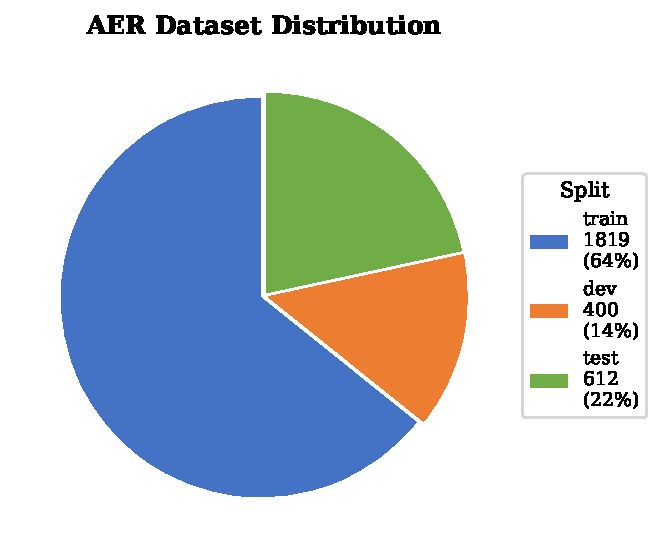
\includegraphics[width=0.75\columnwidth]{figures/data_distribution.pdf}
    \caption{AER data distribution across splits.}
    \label{fig:data_dist}
\end{figure}

As shown in Figure~\ref{fig:data_dist}, the dataset is partitioned into training (1,819 instances, 64\%), development (400 instances, 14\%), and test (612 instances, 22\%) splits. The instances are organized around 36 distinct topics in training, 8 in development, and 12 in testing, spanning domains such as politics, finance, and public emergencies. Each topic is associated with approximately 10 retrieved documents, providing background context for the events.

\begin{table}[t]
\centering
\small
\begin{tabular}{lrrrr}
\toprule
\textbf{Split} & \textbf{Questions} & \textbf{Topics} & \textbf{Single} & \textbf{Multi} \\
\midrule
Train & 1,819 & 36 & 1,042 & 777 \\
Dev & 400 & 8 & -- & -- \\
Test & 612 & 12 & -- & -- \\
\bottomrule
\end{tabular}
\caption{Dataset statistics. ``Single'' and ``Multi'' refer to instances with single versus multiple correct answers. In training, 42.7\% of instances have multiple correct answers.}
\label{tab:data_stats}
\end{table}

A notable characteristic of this dataset, as shown in Table~\ref{tab:data_stats} and Figure~\ref{fig:answer_dist}, is the prevalence of multi-label instances. In the training set, 777 instances (42.7\%) have multiple correct answers, making this a challenging multi-label classification problem. This distribution motivates our choice of binary cross-entropy loss and threshold optimization, as discussed in Section~\ref{sec:training}.

\begin{figure}[t]
    \centering
    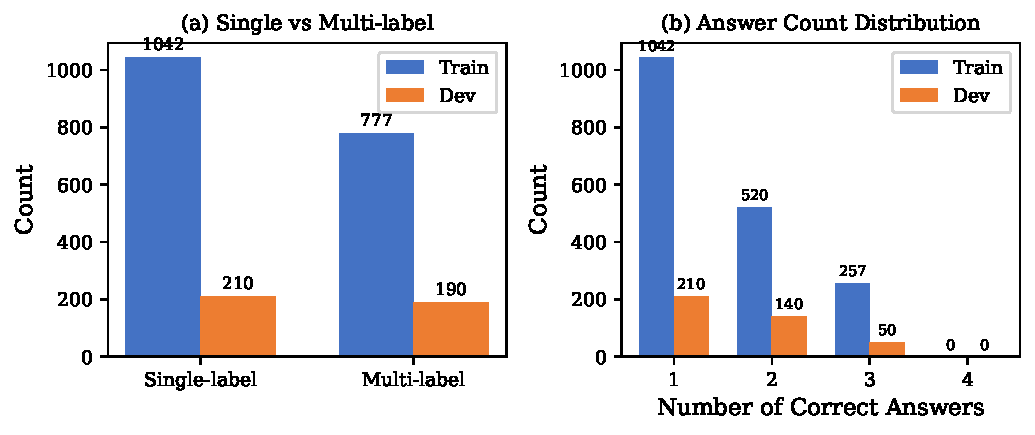
\includegraphics[width=\columnwidth]{figures/answer_distribution.pdf}
    \caption{Answer distribution in the training set: (a) single versus multi-label instances; (b) number of correct answers per instance.}
    \label{fig:answer_dist}
\end{figure}

System performance is evaluated at the instance level using a partial matching scheme. A prediction receives full credit (1.0) if it exactly matches the gold labels, partial credit (0.5) if it is a proper subset of the gold labels, and no credit (0.0) otherwise. This evaluation metric rewards both precision (avoiding incorrect predictions) and recall (capturing all correct answers).

\section{System Overview}

Our system employs a retrieval-augmented architecture with a discriminative classification head. Figure~\ref{fig:system} illustrates the overall pipeline. Compared to pure prompting approaches that rely on zero-shot generation, our approach fine-tunes the model with a multi-label head optimized specifically for this task. We find this discriminative approach substantially outperforms generative alternatives in our experiments (see Appendix~\ref{app:architecture}).

\begin{figure*}[t]
\centering
\resizebox{0.95\textwidth}{!}{
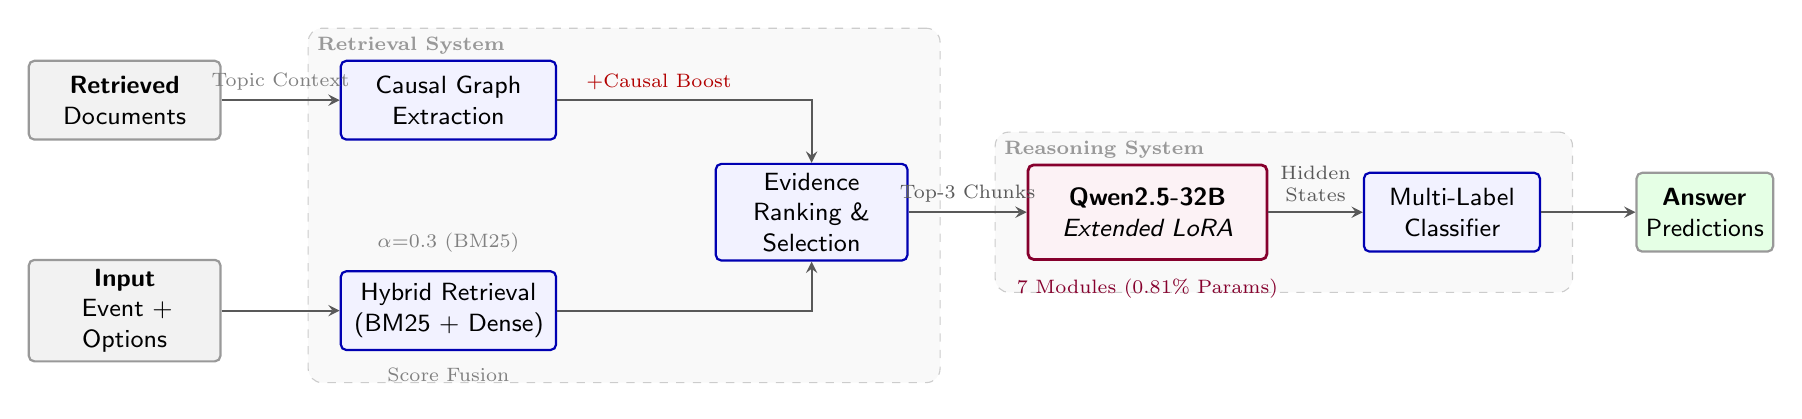
\begin{tikzpicture}[
    node distance=1cm and 1cm,
    font=\small\sffamily,
    block/.style={rectangle, draw=gray!80, fill=white, text width=2.2cm, text centered, minimum height=1.0cm, rounded corners=2pt, line width=0.8pt},
    process/.style={rectangle, draw=blue!70!black, fill=blue!5, text width=2.5cm, text centered, minimum height=1.0cm, rounded corners=2pt, line width=0.8pt},
    model/.style={rectangle, draw=purple!70!black, fill=purple!5, text width=2.8cm, text centered, minimum height=1.2cm, rounded corners=2pt, line width=1pt},
    arrow/.style={->, >=stealth, thick, color=gray!70!black},
    group/.style={rectangle, draw=gray!40, dashed, inner sep=0.4cm, rounded corners=5pt, fill=gray!5}
]

% === INPUTS ===
\node[block, fill=gray!10] (docs) {\textbf{Retrieved}\\Documents};
\node[block, below=1.5cm of docs, fill=gray!10] (query) {\textbf{Input}\\Event + Options};

% === RETRIEVAL MODULE ===
\node[process, right=1.5cm of docs] (graph) {Causal Graph\\Extraction};
\node[process, right=1.5cm of query] (search) {Hybrid Retrieval\\(BM25 + Dense)};

% === FUSION ===
\node[process, right=2cm of search, yshift=1.25cm, text width=2.2cm] (fusion) {Evidence\\Ranking \& Selection};

% === GENERATION MODULE ===
\node[model, right=1.5cm of fusion] (llm) {\textbf{Qwen2.5-32B}\\\textit{Extended LoRA}};
\node[process, right=1.2cm of llm, text width=2cm] (head) {Multi-Label\\Classifier};
\node[block, right=1.2cm of head, fill=green!10, text width=1.5cm] (output) {\textbf{Answer}\\Predictions};

% === GROUPS ===
\begin{pgfonlayer}{background}
    \node[group, fit=(graph) (search) (fusion), label={[anchor=north west, color=gray!80, font=\scriptsize\bfseries]north west:Retrieval System}] (retrieval_group) {};
    \node[group, fit=(llm) (head), label={[anchor=north west, color=gray!80, font=\scriptsize\bfseries]north west:Reasoning System}] (reasoning_group) {};
\end{pgfonlayer}

% === CONNECTIONS ===
% Docs Flow
\draw[arrow] (docs) -- node[above, font=\scriptsize, color=gray] {Topic Context} (graph);
\draw[arrow] (graph) -| node[above, pos=0.2, font=\scriptsize, color=red!70!black] {+Causal Boost} (fusion);

% Query Flow
\draw[arrow] (query) -- (search);
\draw[arrow] (search) -| (fusion);

% Fusion to Model
\draw[arrow] (fusion) -- node[above, font=\scriptsize] {Top-3 Chunks} (llm);

% Model predictions
\draw[arrow] (llm) -- node[above, font=\scriptsize, text width=1.5cm, align=center] {Hidden\\States} (head);
\draw[arrow] (head) -- (output);

% Additional annotations
\node[above=0.1cm of search, font=\scriptsize, color=gray] {$\alpha$=0.3 (BM25)};
\node[below=0.1cm of search, font=\scriptsize, color=gray] {Score Fusion};

\node[below=0.1cm of llm, font=\scriptsize, color=purple!70!black] {7 Modules (0.81\% Params)};

\end{tikzpicture}
}
\caption{\textbf{Overview of the CausalRAG Architecture.} The system consists of two main stages: (1) A \textit{Retrieval System} that enhances standard hybrid search (BM25 + Dense) with domain-specific causal graph extraction to boost causally relevant evidence. (2) A \textit{Reasoning System} based on Qwen2.5-32B fine-tuned with Extended LoRA, which processes the retrieved context to predict the most plausible causes via a multi-label classification head.}
\label{fig:system}
\end{figure*}

The core techniques underlying our system are (i) causal graph extraction for retrieval boosting (\S\ref{sec:causal}), (ii) hybrid retrieval combining BM25 and dense scoring (\S\ref{sec:hybrid}), and (iii) extended LoRA fine-tuning with development set refinement (\S\ref{sec:lora}). We describe each component in detail below.

\subsection{Causal Graph Builder}
\label{sec:causal}

The first stage of our pipeline extracts explicit causal relations from the retrieved documents using pattern matching. We compile a set of regular expressions that capture common causal language patterns: ``X \textit{caused} Y,'' ``X \textit{led to} Y,'' ``X \textit{resulted in} Y,'' ``\textit{because of} X, Y,'' and temporal markers such as ``\textit{after} X, Y'' and ``\textit{following} X, Y.''

For each document, we apply these patterns to extract (cause, effect) pairs, which together form a causal graph associated with the topic. The extracted causal edges serve two purposes. First, they provide explicit causal knowledge that can be summarized in the context provided to the model. Second, and more importantly, they inform our retrieval strategy: document chunks containing extracted causal edges receive a boosted retrieval score (multiplied by a factor of 1.5), prioritizing evidence with explicit causal language.

\subsection{Hybrid Retrieval}
\label{sec:hybrid}

Retrieval-augmented approaches have shown strong performance across a variety of knowledge-intensive NLP tasks \cite{lewis2020rag,guu2020realm}. For abductive reasoning, effective retrieval is particularly important because the correct answer often depends on background knowledge that may be mentioned only briefly in the source documents.

We observe that causal reasoning requires both \textit{explicit keyword matching} and \textit{semantic understanding}. Explicit causal markers such as ``caused,'' ``triggered,'' or ``led to'' are valuable signals that may be missed by purely semantic retrievers. Conversely, implicit causal relations require understanding meaning beyond surface-level lexical overlap. To address this, we combine two complementary retrieval methods using weighted scoring:
\begin{equation}
    s_{\text{hybrid}} = \alpha \cdot \hat{s}_{\text{BM25}} + (1-\alpha) \cdot \hat{s}_{\text{dense}}
\end{equation}
where $\hat{s}$ denotes normalized scores and $\alpha = 0.3$ in our experiments. BM25 \cite{robertson2009probabilistic} provides fast lexical matching that captures explicit causal keywords, while dense retrieval using Sentence-BERT \cite{reimers2019sentence,gao2021simcse,zhang2022mcse} captures semantic similarity beyond lexical overlap. Documents are chunked into segments of approximately 300 characters with 50-character overlap, and we retrieve the top-$k$ chunks (with $k=3$).

\subsection{Extended LoRA Fine-tuning}
\label{sec:lora}

We fine-tune Qwen2.5-32B-Instruct \cite{qwen2024} using QLoRA \cite{dettmers2023qlora} with 4-bit quantization. Standard LoRA \cite{hu2022lora} and adapters \cite{houlsby2019parameter} adapt pre-trained models by adding low-rank decomposition matrices to the attention layers while keeping the original weights frozen. This approach dramatically reduces the number of trainable parameters while maintaining competitive performance.

In our experiments, we extend the standard LoRA configuration to include not only the attention projection layers but also the MLP layers. Specifically, we target seven modules in total: the attention projections (\texttt{q\_proj}, \texttt{k\_proj}, \texttt{v\_proj}, \texttt{o\_proj}) and the feedforward projections (\texttt{gate\_proj}, \texttt{up\_proj}, \texttt{down\_proj}). This results in 268 million trainable parameters, representing only 0.81\% of the total 33 billion parameters. We hypothesize that for tasks requiring complex reasoning, the MLP layers play a crucial role in transforming and combining information.

The classification head consists of a two-layer MLP with GELU activation and dropout, taking the last token's hidden state as input and producing four independent logits (one for each answer option). We train with binary cross-entropy loss to handle the multi-label nature of the task. Gradient checkpointing is enabled to fit the model in 80GB VRAM.

\subsection{Development Set Fine-tuning}
\label{sec:training}

After training on the training set for 2 epochs with gradient accumulation of 32, we select the checkpoint with the highest validation score. However, we observe that the 400 development instances contain valuable signal that is otherwise ``wasted'' during model selection. To leverage this data, we perform one additional epoch of training on the development set with a halved learning rate ($5 \times 10^{-5}$ instead of $10^{-4}$). This technique is motivated by the two-phase training scheme proposed by \citet{zhu2023weaker} and domain adaptation principles \cite{gururangan2020dont}, where training on noisy data first followed by clean data improves performance.

\section{Experimental Setup}

\textbf{Hardware and Training.} All experiments are conducted on a single NVIDIA H100 80GB GPU. Training the 32B model requires approximately 6--8 hours, including 2 epochs on training data. Memory is managed through gradient checkpointing and 4-bit quantization, which together reduce VRAM usage to approximately 70--75GB.

\textbf{Hyperparameters.} We set the LoRA rank to 32 with $\alpha = 64$ and dropout of 0.05. The learning rate is $10^{-4}$ with linear warmup over 10\% of training steps. Maximum sequence length is 384 tokens. Gradient clipping is applied at 0.5 for stability. These hyperparameters were selected based on preliminary experiments on the development set.

\textbf{Baseline.} Our baseline system uses DeBERTa-v3-large \cite{he2021deberta} with a multi-label classification head, trained with binary cross-entropy loss. This baseline achieves 0.63 on the official evaluation.

\section{Results and Analysis}

\subsection{Development Set Performance}

Table~\ref{tab:dev_results} presents the performance of our system variants on the development set. We observe that model scaling provides the largest gain, with Qwen-7B achieving 0.88 compared to the DeBERTa baseline at 0.67. Adding extended LoRA target modules and hybrid retrieval further improves performance. Our best configuration achieves 0.9363 on the development set.

\begin{table}[t]
\centering
\small
\begin{tabular}{lcc}
\toprule
\textbf{System} & \textbf{Dev} & \textbf{$\Delta$} \\
\midrule
DeBERTa Baseline & 0.67 & -- \\
+ Dense RAG & 0.76 & +0.09 \\
+ Causal Graph Boost & 0.80 & +0.04 \\
+ Hybrid (BM25) & 0.82 & +0.02 \\
\midrule
Qwen-7B + QLoRA & 0.88 & +0.06 \\
Qwen-32B + QLoRA & 0.89 & +0.01 \\
+ Extended LoRA & 0.92 & +0.03 \\
+ Dev Fine-tuning & \textbf{0.9363} & +0.02 \\
\bottomrule
\end{tabular}
\caption{Development set performance (AER score). Each row adds one component to the previous configuration.}
\label{tab:dev_results}
\end{table}

\begin{figure}[t]
\centering
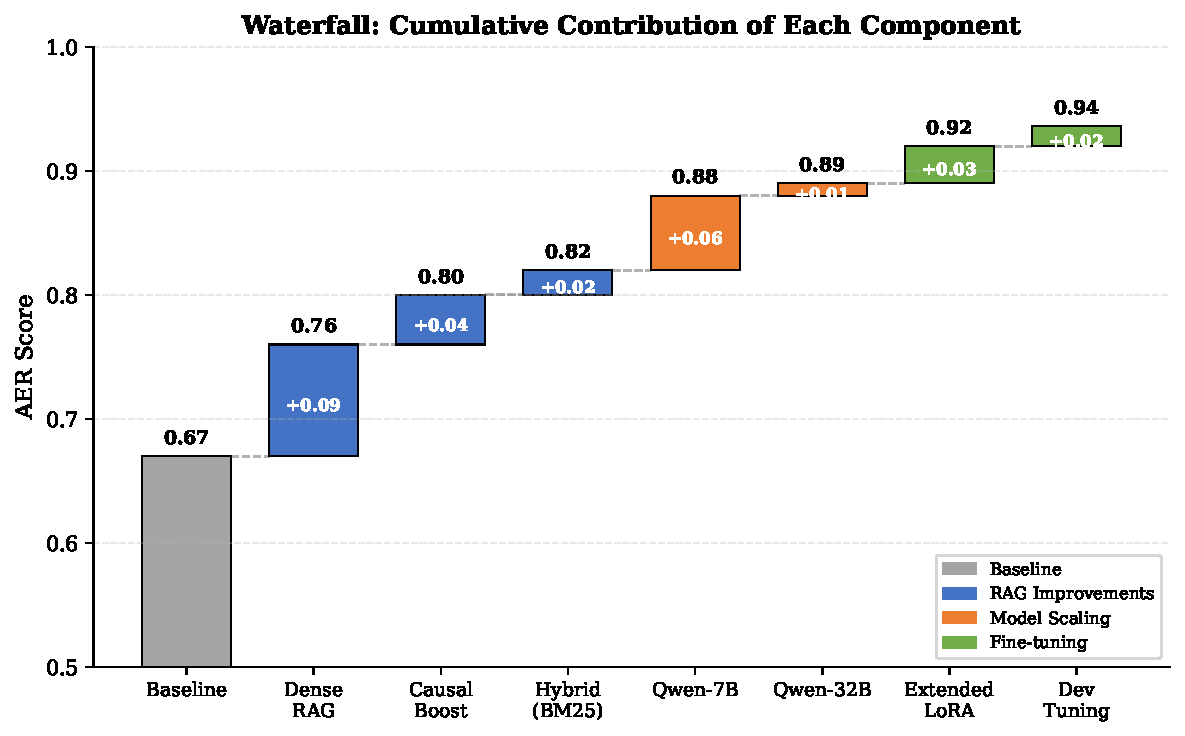
\includegraphics[width=\columnwidth]{figures/ablation_waterfall.pdf}
\caption{Waterfall chart showing the cumulative contribution of each component to the final Development score of 0.9363.}
\label{fig:ablation}
\end{figure}

\subsection{Official Test Set Results}

Table~\ref{tab:results} presents our five official submissions to the shared task. Our progression from baseline to final system illustrates the contribution of each technique.

\begin{table}[t]
\centering
\small
\begin{tabular}{llc}
\toprule
\textbf{System} & \textbf{Key Feature} & \textbf{Test} \\
\midrule
DeBERTa Baseline & Multi-label BCE & 0.63 \\
CausalRAG-7B & +QLoRA, +Hybrid RAG & 0.86 \\
Full SOTA (7B) & +Label Powerset & 0.87 \\
CausalRAG-32B & +Model Scaling & 0.88 \\
\textbf{Extended LoRA} & \textbf{+MLP modules} & \textbf{0.90} \\
\bottomrule
\end{tabular}
\caption{Official test set results for our five submissions. The Extended LoRA configuration achieves the best score of 0.90.}
\label{tab:results}
\end{table}

The DeBERTa baseline establishes a starting point of 0.63. Scaling to Qwen2.5-7B with QLoRA and adding hybrid retrieval yields a dramatic improvement to 0.86, a gain of 23 points. Further refinements through label powerset classification and 32B model scaling provide incremental gains. Our final system with extended LoRA achieves 0.90, representing a total improvement of 27 points over the baseline.

\subsection{Official Leaderboard Comparison}

Table~\ref{tab:leaderboard} presents the final official competition leaderboard. Our system (team name: \textit{WinnerHere} / HCMUS\_RepeatedGames) achieved a high score of 0.90, ranking \textbf{tied for fifth} among all participating teams.

\begin{table}[t]
\centering
\small
\begin{tabular}{clc}
\toprule
\textbf{Rank} & \textbf{Team} & \textbf{Score} \\
\midrule
\textbf{1} & \textbf{nickaraf} & \textbf{0.95} \\
2 & zayme & 0.94 \\
3 & ytachioka & 0.91 \\
3 & pamekalws & 0.91 \\
5 & essiez & 0.90 \\
5 & \textbf{HCMUS\_RepeatedGames (Ours)} & \textbf{0.90} \\
7 & yterao & 0.89 \\
\bottomrule
\end{tabular}
\caption{Official final leaderboard of the top participating teams. Our system achieves a score of 0.90, placing us in a tie for 5th overall.}
\label{tab:leaderboard}
\end{table}

\subsection{Analysis: The Importance of Model Scale}

\begin{figure}[t]
    \centering
    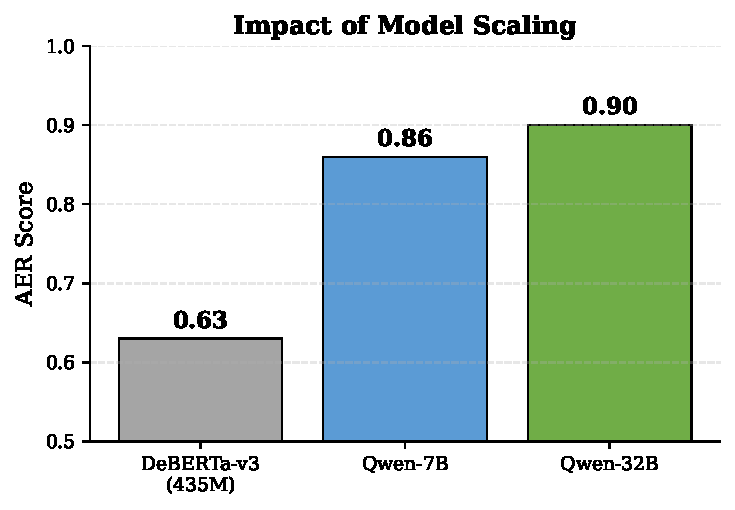
\includegraphics[width=0.95\columnwidth]{figures/model_scaling.pdf}
    \caption{Impact of model scaling on AER test performance. Red arrows show incremental gains: +0.23 from DeBERTa to 7B, +0.04 from 7B to 32B. Annotations indicate the fine-tuning approach used. Total improvement: +0.27.}
    \label{fig:scaling}
\end{figure}

Figure~\ref{fig:scaling} illustrates the dramatic impact of model scaling on this task. Scaling from DeBERTa-v3-large (435M parameters) to Qwen-32B yields a total improvement of 27 points---by far the largest factor in our system's performance.

An important finding is that fine-tuning dominates zero-shot prompting even at large scales. In our experiments, a \textit{fine-tuned} 7B model (0.86) substantially outperforms a \textit{zero-shot} 32B model (0.70) by 16 points. This demonstrates that task-specific adaptation remains essential for abductive reasoning, even when using the largest available models. The complexity of causal inference and the need for evidence-based reasoning appear to exceed what can be accomplished through in-context learning alone.

\subsection{Failed Experiments}

We also report techniques that did not improve performance in our experiments. Multi-hop reasoning, where we traverse the causal graph to find 2-hop causal paths, provided no improvement (0.78 $\rightarrow$ 0.78), suggesting that direct causality is sufficient for this task. A multi-agent debate approach, where multiple model instances debate candidate answers, substantially hurt performance (0.59). Zero-shot prompting with smaller models (7B) achieved only 0.28--0.30.

\section{Conclusion}

We presented CausalRAG, a system achieving 0.90 on SemEval-2026 Task 12 through hybrid retrieval and extended LoRA fine-tuning. Our analysis reveals that model scaling is the dominant factor in performance, contributing 23 of the 27 points of improvement over our baseline. Secondary contributions come from hybrid retrieval (which captures both explicit causal keywords and semantic similarity) and extended LoRA (which trains 7 modules including MLP layers with only 0.81\% of parameters). We demonstrated that fine-tuned smaller models substantially outperform zero-shot larger models, highlighting the continued importance of task-specific adaptation for complex reasoning tasks.

\section*{Limitations}

Our system requires substantial computational resources that may not be accessible to all researchers: an H100 80GB GPU and 6--8 hours of training time. The approach may not generalize to domains outside the training distribution without additional adaptation. Additionally, our development set fine-tuning strategy, while effective for maximizing leaderboard performance, could be considered a form of test set contamination if the validation distribution differs significantly from the test set.

\section*{Acknowledgments}

We thank the SemEval-2026 Task 12 organizers for providing the dataset and evaluation infrastructure.

\bibliography{custom}
% \bibliographystyle{acl_natbib}

\appendix

\section{Model and Architecture Selection}
\label{app:architecture}

In our preliminary study, we examined the capacity of different pre-trained models with and without task-specific training. Table~\ref{tab:model_selection} shows the results.

\begin{table}[h]
\centering
\small
\begin{tabular}{lcc}
\toprule
\textbf{Model} & \textbf{Zero-shot} & \textbf{Fine-tuned} \\
\midrule
DeBERTa-v3-large & -- & 0.63 \\
Qwen2.5-7B & 0.28 & 0.86 \\
Qwen2.5-32B & 0.70 & 0.90 \\
\bottomrule
\end{tabular}
\caption{Comparison of zero-shot vs. fine-tuned performance on the test set.}
\label{tab:model_selection}
\end{table}

We observe that zero-shot performance with smaller models is extremely poor (0.28 for 7B), while even the 32B model in zero-shot setting (0.70) underperforms a fine-tuned 7B model (0.86). This confirms that task-specific adaptation is essential for this task, regardless of model scale.

\section{Hyperparameter Configuration}
\label{app:hyperparams}

Table~\ref{tab:hyperparams} shows the complete hyperparameter configuration for our best system.

\begin{table}[h]
\centering
\small
\begin{tabular}{ll}
\toprule
\textbf{Parameter} & \textbf{Value} \\
\midrule
\multicolumn{2}{l}{\textit{Model Configuration}} \\
Base Model & Qwen2.5-32B-Instruct \\
Quantization & 4-bit NF4 \\
Hidden Size & 5,120 \\
Total Parameters & 33.0B \\
Trainable Parameters & 268M (0.81\%) \\
\midrule
\multicolumn{2}{l}{\textit{LoRA Configuration}} \\
LoRA Rank ($r$) & 32 \\
LoRA Alpha ($\alpha$) & 64 \\
LoRA Dropout & 0.05 \\
Target Modules & \texttt{q,k,v,o,gate,up,down} \\
\midrule
\multicolumn{2}{l}{\textit{Training Configuration}} \\
Learning Rate & $1 \times 10^{-4}$ \\
Batch Size & 1 \\
Gradient Accumulation & 32 \\
Epochs & 2 \\
Warmup Ratio & 0.1 \\
Gradient Clipping & 0.5 \\
Gradient Checkpointing & Enabled \\
\midrule
\multicolumn{2}{l}{\textit{RAG Configuration}} \\
Chunk Size & 300 chars \\
Chunk Overlap & 50 chars \\
Top-K Chunks & 3 \\
Max Context & 1,000 chars \\
BM25 Weight ($\alpha$) & 0.3 \\
Dense Weight ($1{-}\alpha$) & 0.7 \\
Causal Edge Boost & 1.5$\times$ \\
\bottomrule
\end{tabular}
\caption{Complete hyperparameter configuration.}
\label{tab:hyperparams}
\end{table}

\section{Causal Pattern Extraction}
\label{app:patterns}

Table~\ref{tab:patterns} lists the regular expression patterns used for extracting causal relations from documents. These patterns are designed to capture common English causal constructions.

\begin{table}[h]
\centering
\small
\begin{tabular}{ll}
\toprule
\textbf{Pattern} & \textbf{Type} \\
\midrule
\texttt{(.+?) caused (.+)} & CAUSE \\
\texttt{(.+?) led to (.+)} & CAUSE \\
\texttt{(.+?) resulted in (.+)} & CAUSE \\
\texttt{(.+?) triggered (.+)} & CAUSE \\
\texttt{(.+?) prompted (.+)} & CAUSE \\
\texttt{because of (.+?), (.+)} & CAUSE \\
\texttt{after (.+?), (.+)} & TEMPORAL \\
\texttt{following (.+?), (.+)} & TEMPORAL \\
\bottomrule
\end{tabular}
\caption{Causal patterns for graph extraction.}
\label{tab:patterns}
\end{table}

\section{Full Experiment Results}
\label{app:full_results}

Table~\ref{tab:full_results} presents all our submitted experiments to the shared task leaderboard.

\begin{table}[h]
\centering
\small
\begin{tabular}{llc}
\toprule
\textbf{ID} & \textbf{Method} & \textbf{Score} \\
\midrule
\multicolumn{3}{l}{\textit{Top Performers (Score $\geq$ 0.85)}} \\
485547 & 32B + Extended LoRA + Hybrid & \textbf{0.90} \\
485240 & 32B + Dev Tuning & 0.88 \\
484482 & 32B + QLoRA & 0.88 \\
484738 & Full SOTA (7B) & 0.87 \\
484742 & Self-RAG Gating & 0.86 \\
483875 & 7B + QLoRA & 0.86 \\
\midrule
\multicolumn{3}{l}{\textit{Mid-Range (Score 0.70--0.84)}} \\
484890 & 32B Initial & 0.82 \\
483161 & CausalRAG (DeBERTa) & 0.78 \\
483231 & CF-RAG & 0.76 \\
482886 & Contrastive + RAG & 0.74 \\
482860 & Qwen-32B Zero-shot & 0.70 \\
\midrule
\multicolumn{3}{l}{\textit{Low Performers (Score $<$ 0.70)}} \\
482526 & DeBERTa Baseline & 0.63 \\
483392 & Multi-Agent + RAG & 0.59 \\
482846 & CISC & 0.30 \\
482849 & PC-SubQ & 0.28 \\
\bottomrule
\end{tabular}
\caption{Full experiment results from the leaderboard.}
\label{tab:full_results}
\end{table}

\section{Reproducibility}
\label{app:code}

Our complete training code is provided below for reproducibility. This code is designed to run on Kaggle with a single H100 80GB GPU.

\begin{verbatim}
# Key configuration for Kaggle
MODEL_NAME = 'Qwen/Qwen2.5-32B-Instruct'
LORA_R = 32
LORA_ALPHA = 64
LORA_TARGET_MODULES = [
    "q_proj", "k_proj", "v_proj", "o_proj",
    "gate_proj", "up_proj", "down_proj"
]
USE_GRAD_CHECKPOINT = True
BM25_WEIGHT = 0.3
DENSE_WEIGHT = 0.7
CAUSAL_EDGE_BOOST = 1.5
\end{verbatim}

The full code is available at our GitHub repository.

\end{document}
